% main_draft.tex — Full proposal draft, Week 8

\documentclass[12pt]{article}

% --- Packages ---
\usepackage[T1]{fontenc}
\usepackage[utf8]{inputenc}
\usepackage[margin=1in]{geometry}
\usepackage{graphicx}
\usepackage{booktabs}
\usepackage{amsmath}
\usepackage{parskip}
\usepackage{setspace}
\usepackage{enumitem}
\usepackage{hyperref}
 
% --- Bibliography (APA 7th, biblatex + biber) ---
\usepackage[backend=biber, style=apa, sorting=nyt, natbib=true]{biblatex}
\addbibresource{references.bib}
 
% --- Title ---
\title{\textbf{Full Proposal Draft} \\
\large Predicting Attention from the Surface: Movie-Calibrated fNIRS as a Proxy for Whole-Brain fMRI}
\author{Judy Chen \\ MACS 30200: Computational Research Design}
\date{Spring 2026}
 
\begin{document}

\maketitle
\onehalfspacing
 
% --- Abstract ---

% abstract.tex — Full proposal draft, Week 8
% Place this file alongside main_draft.tex and 
% abstract.tex — Full proposal draft, Week 8
% Place this file alongside main_draft.tex and 
% abstract.tex — Full proposal draft, Week 8
% Place this file alongside main_draft.tex and \input{abstract} where needed.

\begin{abstract}

Individual differences in sustained attention predict academic achievement, occupational performance, and vulnerability to clinical conditions, yet the neuroimaging tools best suited to studying these differences are expensive, immobile, and concentrated in well-funded institutions. This project asks whether a brief, portable brain recording session can approximate whole-brain neural measurement without a scanner. Specifically, I test whether functional near-infrared spectroscopy (fNIRS) signals recorded during naturalistic movie-watching can train a computational model that predicts whole-brain fMRI activity, and whether that model generalizes to structured cognitive tasks where it can detect meaningful individual differences in attentional control.

The approach uses adapted principal component regression (aPCR) to learn a linear mapping between 42 fNIRS channels and 122 fMRI brain regions, trained on temporally aligned data from two separate participant groups (N\,=\,28 fNIRS, N\,=\,59 fMRI) who watched the same film. The trained model is then frozen and applied to fNIRS data from cognitive tasks (n-back, Continuous Performance Task) that the model has never encountered. The primary outcome is whether predicted whole-brain activation patterns correlate with behavioral measures of attentional stability, operationalized as intraindividual reaction time variability.

Preliminary results from the movie-watching training phase show that the model significantly predicts 56 of 122 brain regions (FDR $q < 0.05$), with particularly strong performance in the dorsal attention network (11 of 14 ROIs significant) and ventral attention network (14 of 24 ROIs). The predicted inter-subject functional connectivity matrix closely matches the observed fMRI connectivity structure ($r = 0.617$, $p = 0.001$). These results establish the model's capacity to recover large-scale brain organization from surface signals alone, providing the foundation for the cross-task individual differences analyses that follow.

\end{abstract}
 where needed.

\begin{abstract}

Individual differences in sustained attention predict academic achievement, occupational performance, and vulnerability to clinical conditions, yet the neuroimaging tools best suited to studying these differences are expensive, immobile, and concentrated in well-funded institutions. This project asks whether a brief, portable brain recording session can approximate whole-brain neural measurement without a scanner. Specifically, I test whether functional near-infrared spectroscopy (fNIRS) signals recorded during naturalistic movie-watching can train a computational model that predicts whole-brain fMRI activity, and whether that model generalizes to structured cognitive tasks where it can detect meaningful individual differences in attentional control.

The approach uses adapted principal component regression (aPCR) to learn a linear mapping between 42 fNIRS channels and 122 fMRI brain regions, trained on temporally aligned data from two separate participant groups (N\,=\,28 fNIRS, N\,=\,59 fMRI) who watched the same film. The trained model is then frozen and applied to fNIRS data from cognitive tasks (n-back, Continuous Performance Task) that the model has never encountered. The primary outcome is whether predicted whole-brain activation patterns correlate with behavioral measures of attentional stability, operationalized as intraindividual reaction time variability.

Preliminary results from the movie-watching training phase show that the model significantly predicts 56 of 122 brain regions (FDR $q < 0.05$), with particularly strong performance in the dorsal attention network (11 of 14 ROIs significant) and ventral attention network (14 of 24 ROIs). The predicted inter-subject functional connectivity matrix closely matches the observed fMRI connectivity structure ($r = 0.617$, $p = 0.001$). These results establish the model's capacity to recover large-scale brain organization from surface signals alone, providing the foundation for the cross-task individual differences analyses that follow.

\end{abstract}
 where needed.

\begin{abstract}

Individual differences in sustained attention predict academic achievement, occupational performance, and vulnerability to clinical conditions, yet the neuroimaging tools best suited to studying these differences are expensive, immobile, and concentrated in well-funded institutions. This project asks whether a brief, portable brain recording session can approximate whole-brain neural measurement without a scanner. Specifically, I test whether functional near-infrared spectroscopy (fNIRS) signals recorded during naturalistic movie-watching can train a computational model that predicts whole-brain fMRI activity, and whether that model generalizes to structured cognitive tasks where it can detect meaningful individual differences in attentional control.

The approach uses adapted principal component regression (aPCR) to learn a linear mapping between 42 fNIRS channels and 122 fMRI brain regions, trained on temporally aligned data from two separate participant groups (N\,=\,28 fNIRS, N\,=\,59 fMRI) who watched the same film. The trained model is then frozen and applied to fNIRS data from cognitive tasks (n-back, Continuous Performance Task) that the model has never encountered. The primary outcome is whether predicted whole-brain activation patterns correlate with behavioral measures of attentional stability, operationalized as intraindividual reaction time variability.

Preliminary results from the movie-watching training phase show that the model significantly predicts 56 of 122 brain regions (FDR $q < 0.05$), with particularly strong performance in the dorsal attention network (11 of 14 ROIs significant) and ventral attention network (14 of 24 ROIs). The predicted inter-subject functional connectivity matrix closely matches the observed fMRI connectivity structure ($r = 0.617$, $p = 0.001$). These results establish the model's capacity to recover large-scale brain organization from surface signals alone, providing the foundation for the cross-task individual differences analyses that follow.

\end{abstract}

 
% --- Introduction (Big Picture) ---
% introduction.tex — Full proposal draft, Week 8
% Revised from bigpicture.tex (Week 5). Light edits for flow and RQ placement.

\section{Introduction}

Attention is unevenly distributed across populations, and so is our ability to study it. Individual differences in sustained attention and working memory predict a wide range of consequential life outcomes, from academic achievement and occupational performance to vulnerability to clinical conditions like attention-deficit/hyperactivity disorder \citep{kofler2013}. The neuroscientific tools most capable of measuring these differences, however, are expensive, stationary, and concentrated in well-funded research institutions. Functional magnetic resonance imaging (fMRI) scanners cost millions of dollars to purchase and maintain, require specially shielded rooms, and are largely absent from the low-income communities and under-resourced clinical settings where attentional difficulties are most prevalent. As a result, the knowledge base about attention and the brain reflects a structurally skewed sample of who can access a scanner \citep{farah2006}.

This project asks whether that constraint can be relaxed. The central question is whether, if a participant wears a portable brain sensor while watching a movie, the recording from that single naturalistic session can be used to train a computational model that later predicts whole-brain neural activity during structured attention tasks. The portable sensor in question is functional near-infrared spectroscopy (fNIRS), a lightweight headset that measures cortical hemodynamics by detecting changes in light absorption through the scalp. If the approach works, it would allow researchers to approximate fMRI-quality, whole-brain measures of cognitive engagement from a low-cost recording taken in a classroom, a clinic, or a community center, without any scanner access.

The design draws on two datasets linked by a shared naturalistic stimulus, the 1959 Hitchcock film \textit{North by Northwest} (NNW). An ongoing in-lab fNIRS study (N\,=\,28 participants with usable data, spanning participant IDs p01--p34, target N\,=\,40) records oxygenated hemoglobin (HbO) time series from 42 prefrontal, lateral parietal, and temporal-occipital channels while participants watch the film and then complete a series of attention tasks. These tasks include a face-based working memory n-back task at 1-back and 2-back difficulty levels and two rounds of a Continuous Performance Task (CPT). A separate, open fMRI dataset from a collaborating lab (N\,=\,59 different participants) provides fully preprocessed BOLD time series across 122 brain regions from participants who watched the same film in a scanner. Because both groups watched the same movie, their neural responses are temporally aligned even though they are entirely different people. This shared temporal structure is the engine of the approach.

The computational method at the core of the project is adapted principal component regression (aPCR), following \citet{gao2025}. The model first reduces both the fNIRS and fMRI recordings to their most important underlying components via PCA, retaining components capturing 75\% of fNIRS variance (approximately 14 components) and 85\% of fMRI variance (approximately 52 components), matching the thresholds used in the original Gao et al.\ framework. It then uses ordinary least-squares regression to learn the linear mapping between those component spaces. Training uses leave-one-out cross-validation across N\,=\,28 participants. In each fold, 27 fNIRS participants are paired with all 59 fMRI participants (1,593 training pairs), and the held-out fNIRS participant's data are passed through the frozen learned mapping to generate a predicted whole-brain fMRI time series for 122 regions over 886 seconds. The NNW pipeline has been run end-to-end on the full sample. The model significantly predicts 56 of 122 brain regions (FDR-corrected, $q < 0.05$), with particularly strong performance in the dorsal attention network (11/14 ROIs, 79\%) and ventral attention network (14/24 ROIs, 58\%). At the connectivity level, the Pearson correlation between predicted and true inter-subject functional connectivity (ISFC) matrices is $r = 0.617$ ($p = 0.001$, permutation test), which indicates that the model preserves not just local activation patterns but the large-scale organization of brain-wide communication during the film.

The project goes beyond the original \citet{gao2025} framework by reframing the primary question. Rather than asking whether the model can transfer across paradigms in a technical sense, this project poses a social science question: can we detect meaningful individual differences in who pays attention, and can we do so without a scanner? For each cognitive task, the frozen NNW model will be applied to each participant's task fNIRS data to generate predicted whole-brain time series. These predictions will be evaluated for neural plausibility, specifically whether predicted activation patterns in frontoparietal networks exceed default mode network activation during high-load conditions, as the fMRI literature would predict. They will also be evaluated for individual differences, specifically whether per-subject predicted activation patterns correlate with behavioral performance including n-back accuracy, CPT hit rate, and reaction time variability. This is where the equity argument becomes concrete. If a brief, portable, naturalistic recording session can approximate the neural signature of attentional capacity, then rigorous cognitive neuroscience becomes possible in the settings and populations that have historically been excluded from it. Reaction time variability is particularly well-suited as the individual-differences target because it is sensitive enough to discriminate clinical and subclinical attentional profiles, and if the predicted neural patterns track it, the approach offers a path toward accessible, whole-brain-equivalent measures of attentional stability in schools, clinics, and communities where MRI infrastructure simply does not exist.

The project addresses four specific research questions:

\begin{enumerate}
    \item[\textbf{RQ1:}] Does an fNIRS-to-fMRI mapping trained on naturalistic movie-watching generalize to predict whole-brain neural dynamics during structured cognitive tasks (n-back, CPT)?
    \item[\textbf{RQ2:}] Which brain regions maintain reliable fNIRS-to-fMRI mapping across naturalistic and cognitive paradigms, and do these correspond to domain-general attention networks?
    \item[\textbf{RQ3:}] Can the model predict meaningful differences in brain activity between easy and hard working memory conditions, and do those predictions correlate with behavioral performance (accuracy, reaction time variability)?
    \item[\textbf{RQ4:}] Could a single brief movie-watching session serve as a universal calibration paradigm for portable fNIRS, enabling whole-brain-equivalent neurocognitive assessment without a scanner?
\end{enumerate}

This project makes four contributions. First, it provides the first systematic test of whether an fNIRS-to-fMRI mapping trained on naturalistic stimuli generalizes to structured cognitive paradigms without retraining. Second, it introduces a cross-dataset, cross-paradigm validation design that combines a fully processed open fMRI dataset with ongoing portable-sensor data collection, demonstrating a practical template for low-cost neuroimaging research. Third, it targets individual differences in attentional stability as the outcome of interest, grounding the technical test in a consequential social question about who can be measured and where. Fourth, it establishes a concrete equity argument: if the approach succeeds, meaningful whole-brain cognitive neuroscience becomes achievable in schools, clinics, and community settings without MRI infrastructure.

 
% --- Literature Review ---
% litreview_revised.tex — Full proposal draft, Week 8
% Revised from litreview.tex (Week 5). Minor edits for transition into Methods.

\section{Literature Review}

Understanding individual differences in attention has long been a goal of cognitive neuroscience, but studying it rigorously requires measuring the brain. Attention and working memory are among the most consequential cognitive capacities humans possess. They predict academic achievement, occupational performance, and vulnerability to clinical conditions including ADHD, with large and reliable effect sizes across the population \citep{kofler2013}. These capacities are also not randomly distributed. Sustained attention and executive function are meaningfully associated with socioeconomic status, with children from lower-income backgrounds showing consistent disadvantages in working memory and attentional control that are reflected not only in behavior but in the structure and function of prefrontal and hippocampal brain regions \citep{farah2006, noble2015}. The implication is that the populations most affected by attentional difficulties are also the most likely to be excluded from the scientific infrastructure that studies those difficulties. fMRI scanners, the dominant tool for imaging attention in the brain, are expensive, physically fixed, and concentrated in wealthy, Western, academic institutions, which means that research in low- and middle-income countries, non-laboratory community settings, and resource-limited clinical environments is structurally underrepresented \citep{burns2019}. The present project is organized around the question of whether that constraint can be relaxed through the combination of portable neuroimaging and naturalistic experimental design.

Functional near-infrared spectroscopy (fNIRS) is the most promising candidate for portable neuroimaging. It works by shining near-infrared light (typically 650 to 900 nm) through the scalp and detecting changes in the absorption of oxygenated (HbO) and deoxygenated (HbR) hemoglobin in cortical tissue, which is the same hemodynamic signal that fMRI measures, though restricted to cortical surface regions accessible to light \citep{kamran2016}. Unlike fMRI, fNIRS requires no magnetic field or radio-frequency pulses, tolerates participant movement, and can be deployed in any setting without special infrastructure. These properties have allowed it to reach populations and contexts previously inaccessible to neuroimaging. \citet{burns2019} demonstrated that portable fNIRS could measure meaningful individual differences in prefrontal responses to persuasive messages in a native Arabic-speaking sample recruited in Jordan, a population almost entirely absent from social neuroscience, and replicated established findings about medial and ventromedial prefrontal cortex involvement in persuasion. This work directly establishes that fNIRS prefrontal signals are sensitive enough to detect socially meaningful individual differences outside laboratory settings, which is a core assumption of the present project. The limitation fNIRS cannot overcome is depth. It is physically incapable of measuring medial prefrontal cortex, subcortical structures, or any brain region far from the scalp-mounted optodes. Because attention depends on a distributed network that includes the hippocampus, thalamus, basal ganglia, and portions of cingulate cortex, none of which fNIRS can reach, a portable surface-only recording cannot by itself provide the kind of whole-brain picture that motivates research on neural individual differences.

The key insight motivating this project is that the limitation of surface-only measurement does not have to be fatal. Deep brain activity can be inferred from cortical activity through learned functional connectivity relationships. \citet{liu2015} provided early proof of concept by scanning 17 participants simultaneously with fNIRS and fMRI during multiple cognitive tasks and showing that activity in deep structures, including the insula, hippocampus, and caudate, could be significantly predicted from surface cortical fNIRS signals, with top-quintile predictions achieving correlations of approximately $r = 0.70$. The neural basis for this inferential approach is well established: deep and subcortical regions are functionally coupled with surface cortical regions, so their activity tends to rise and fall together. A computational model that has learned what the fMRI signal looks like when the cortical signal looks a certain way can exploit this coupling. The limitation in Liu et al.'s work was the requirement that the same individuals be scanned simultaneously in both modalities, which is expensive, logistically demanding, and ultimately defeats the purpose of building a portable tool. The methodological breakthrough that resolved this came from naturalistic paradigms, which provide a way to align signals across separately scanned participant groups.

The logic of naturalistic alignment rests on a substantial literature on inter-subject correlation (ISC), which refers to the phenomenon whereby independently scanned individuals who experience the same naturalistic stimulus produce temporally synchronized brain responses across a wide network of regions \citep{hasson2004, hasson2010, nastase2019}. When people watch the same film, their auditory cortices respond to dialogue in near-lockstep, their prefrontal regions engage with narrative tension at similar moments, and their default mode networks activate and deactivate in patterns that are recognizably consistent across individuals \citep{hasson2010}. This shared temporal structure is largely absent during structured cognitive tasks, where individual differences in strategy, arousal, and performance introduce person-specific variance that overwhelms the shared signal \citep{nastase2019}. \citet{finn2021} showed that this property of naturalistic stimuli has direct practical consequences: functional connectivity measured during movie watching yields substantially more accurate predictions of trait-level behavioral phenotypes than connectivity measured during rest, with highly social clips producing reliable predictions in under three minutes of data. Naturalistic viewing, in other words, does not merely produce strong shared responses. It also amplifies the behaviorally relevant structure of individual differences in brain organization. For this project, the relevant implication is that a movie-watching session provides the ideal calibration paradigm because the shared temporal structure of the film creates a strong ISC signal that makes it possible to train a cross-dataset mapping between fNIRS and fMRI participants who were never scanned together, while the within-person variability around that shared signal may encode individual cognitive profiles.

\citet{gao2025} operationalized this insight in the aPCR framework. By training an adapted principal component regression model on fNIRS and fMRI data collected during naturalistic TV episode viewing, across separate participant groups who watched the same content, they demonstrated that whole-brain fMRI dynamics could be significantly predicted from prefrontal surface signals alone in 66 of 122 brain regions ($q < 0.05$), including subcortical and medial regions physically inaccessible to fNIRS. The model also generalized to an independent naturalistic dataset recorded during a different TV series, establishing that the learned cross-modal mapping captures stimulus-general structure rather than overfitting to one particular narrative \citep{gao2025}. The Gao et al.\ framework was designed and tested entirely within naturalistic paradigms, with both training and test data coming from movie or TV episode viewing. The present project takes the harder step of asking whether a model calibrated on naturalistic data can transfer to structured cognitive tasks, where the stimulus-driven ISC that supported model training is largely absent. This is the key untested assumption, and the answer to it determines whether naturalistic calibration can serve as a general-purpose tool for portable neurocognitive assessment.

Evaluating whether the cross-task transfer is meaningful requires a framework for what meaningful brain predictions during attention tasks should look like. Two intersecting literatures are relevant here. First, there is strong evidence that the frontoparietal network, and particularly the dorsal attention network (DAN) and the cognitive control network (CONT), functions as a set of flexible hubs whose global connectivity patterns shift more dramatically across task demands than any other network in the brain \citep{cole2013}. In a study spanning 64 different cognitive tasks, \citet{cole2013} found that frontoparietal regions could identify the current task from their connectivity patterns alone, and that this held even for tasks the person had never practiced before, which suggests that these hubs encode task demands in a generalizable format. Because the fNIRS cap used in this project covers precisely these prefrontal and lateral parietal regions, the model has direct access to the surface signals most likely to encode task-relevant structure. Building on this, \citet{braun2015} showed in 344 participants that how much frontal networks reorganized their communication patterns during the n-back task predicted both working memory accuracy and scores on external neuropsychological measures of cognitive flexibility, suggesting that individual differences in frontal system reconfiguration during a cognitive challenge carry behavioral consequences that generalize well beyond the task itself. This finding bears directly on Phase 5 of the present project: if the aPCR-predicted brain patterns preserve this frontoparietal reconfiguration structure, they should correlate with behavioral performance on the n-back and CPT. More broadly, \citet{tavor2016} demonstrated in the Human Connectome Project that task-evoked brain activity during seven different cognitive paradigms could be accurately predicted from resting-state connectivity alone, without any task data from the individuals being predicted. The parallel to the present project is close. Just as resting-state connectivity encodes something like a neural blueprint for how a person will respond to cognitive demands, a naturalistic fNIRS session may encode enough of an individual's brain organization to allow meaningful predictions of their task-evoked dynamics.

The second relevant literature addresses how behavioral performance during cognitive tasks can be used to index the quality of attention regulation. Reaction time variability (RTV) refers to the trial-to-trial inconsistency in how quickly a person responds across a sustained performance task, and it is among the most robust behavioral markers of attentional control. A meta-analysis of 319 studies by \citet{kofler2013} found that individuals with ADHD showed significantly greater RTV than typically developing peers (Hedges' $g = 0.76$ for children, $g = 0.46$ for adults). This elevation was more discriminating than mean response speed, persisted across task types including the n-back and CPT, and was substantially reduced by stimulant treatment ($g = -0.74$) but unaffected by behavioral interventions. The choice of RTV as the primary individual-differences index in this project, rather than task accuracy or mean response time, is deliberate. Accuracy is susceptible to floor and ceiling effects: in healthy young adults, 1-back performance is near-perfect and fails to differentiate individuals. Mean reaction time, for its part, conflates speed-accuracy tradeoffs with attentional stability. RTV, by contrast, captures moment-to-moment fluctuations in the efficiency of cognitive processing and remains discriminating even when average performance is high, because it reflects the regularity of attentional engagement across trials rather than its central tendency. Critically, RTV is not a marker only of clinical disorder. \citet{macdonald2009} reviewed evidence suggesting that intraindividual variability in cognitive performance tracks the health and efficiency of underlying neural systems, specifically the stability of dopaminergic neuromodulation, the integrity of white matter connectivity, and the regulatory strength of prefrontal cortex, and that these relationships hold across the full range of healthy adults. The theoretical account connecting RTV to brain dynamics was provided by \citet{sonugabarke2007}, who proposed the default mode interference hypothesis. During goal-directed tasks, the default mode network (DMN) is normally suppressed to allow task-relevant networks to operate without competition. When this suppression fails periodically, the DMN briefly reactivates and disrupts processing of the current stimulus, producing an attentional lapse that manifests as an unusually slow response on that trial. High RTV is, on this account, a behavioral fingerprint of poor DMN suppression. The DMN is also one of the networks where the aPCR model shows strong fNIRS-to-fMRI predictions (7 of 26 ROIs significant), which creates a testable prediction for the present project: participants with higher RTV should show more intrusion of rest-like, DMN-active dynamics during their task fNIRS recordings, making their task signals structurally different from movie-watching signals and potentially altering the model's ability to generate meaningful task-period predictions.

Taken together, these three bodies of literature converge on the design of the present project and jointly justify its specific choices. The fNIRS-to-fMRI translation literature establishes the computational feasibility of cross-modal inference from cortical surface signals. The naturalistic paradigm literature explains why a movie provides the ideal training context: it generates the inter-subject correlation necessary for cross-dataset model training and amplifies individual variation in brain organization in ways that resting-state recordings do not \citep{finn2021, gao2025, hasson2010}. The RTV literature links a simple behavioral measure, one that requires no imaging at all, to the neural dynamics the model is trying to predict, providing a concrete individual-differences target for evaluating whether the cross-task predictions are behaviorally meaningful \citep{kofler2013}. The equity framing is not rhetorical. The same reason the project uses movie-watching rather than fMRI, namely that it requires no scanner, is the reason the approach could matter beyond this study. If a brief, passive, naturalistic fNIRS session produces predictions that correlate with attentional performance, then the field has a candidate method for conducting whole-brain-equivalent attention research in schools, clinics, and communities where MRI access is not available. These are precisely the settings and populations that the existing literature, with its structural dependence on scanner infrastructure, has historically excluded \citep{burns2019, farah2006, noble2015}. What follows describes how the two datasets are combined and analyzed to test whether that candidate method delivers.

 
% --- Methods and Data ---
% methods.tex — Full proposal draft, Week 8
% Revised per grader feedback: new section structure (Experiment Design), Participants,
% Stimuli, Procedures, Attention Check, Manipulation Check subsections added.
% Updated N=28, PCA 75%/85%, training pairs=1,593.

\section{Experiment Design}

\subsection{Data Collection}

The project draws on two separate datasets, linked by a shared movie stimulus: the 1959 Hitchcock film \textit{North by Northwest} (NNW).

\paragraph{fNIRS data (ongoing collection, target N\,=\,40).} Each participant comes in for a single session and completes all tasks in the following fixed order: (1) the NNW movie-watching block; (2) CPT session~1 immediately followed by CPT-MEM session~1; (3) the n-back task; and (4) CPT session~2 immediately followed by CPT-MEM session~2. We currently have 28 participants with usable data (spanning participant IDs p01--p34). fNIRS is recorded with a NIRSport2 system using a 50-channel cap (42 standard channels plus 8 short-separation channels) that detects cortical surface activity via near-infrared light. Files are stored in SNIRF format and synced with task events via Lab Streaming Layer (LSL) triggers. The 42 standard channels cover bilateral prefrontal, lateral temporal-parietal, and superior posterior cortex, with no coverage over primary visual cortex. Behavioral data, including n-back accuracy, CPT hit rates, false alarm rates, reaction times, and CPT-MEM recognition confidence ratings, are recorded alongside the fNIRS via PsychoPy and serve as the outcome variables for the individual differences analyses.

\paragraph{fMRI data (open dataset, N\,=\,59).} A publicly available dataset from a collaborating lab provides the fMRI ground truth for model training: 59 participants who watched the same NNW film in an MRI scanner, yielding fully preprocessed BOLD time series across 122 brain regions (59 subjects $\times$ 122 ROIs $\times$ 886 timepoints), parcellated using a combined Yeo 17-network, Brainnetome, and subcortical atlas. These preprocessed files are fully denoised AFNI outputs (\texttt{errts.tproject.nii}). No further data collection or permissions are needed for this component.

Because the two groups of participants watched the same movie, their brain responses are temporally aligned even though they are completely different people. After trimming for preprocessing differences (the fMRI pipeline removes the first 3 seconds of video, so fMRI volume 1 corresponds to movie second 4), there are 886 seconds of shared signal to work with. Crucially, the fact that the participants are different individuals means the model has to learn generalizable, stimulus-driven patterns rather than anything person-specific.

\subsection{Participants}

Thirty-four participants were enrolled (participant IDs p01--p34). Six were excluded due to persistent bad optode contact or excessive motion artifacts, yielding an analytic sample of N\,=\,28 (mean age\,=\,20.4 years, SD\,=\,0.8, range\,=\,18.9--22.5; 16 male, 12 female). Racial and ethnic composition: White ($n\,=\,11$), Asian ($n\,=\,6$), Hispanic or Latino ($n\,=\,4$), Other ($n\,=\,4$), Black or African American ($n\,=\,3$). Participants were recruited from the University of Chicago undergraduate population, compensated with course credit or payment, and provided written informed consent under a protocol approved by the University of Chicago IRB.

\subsection{Stimuli}

\paragraph{Movie stimulus.} The shared naturalistic stimulus is an 886-second clip from \textit{North by Northwest} (Alfred Hitchcock, 1959). This film was selected for two reasons: (1) it is the same stimulus used by the open fMRI dataset, enabling temporal alignment of neural responses across independent participant groups; and (2) it is a commercially released narrative film with complex audiovisual content, known from the ISC literature to drive reliable, distributed neural responses across viewers \citep{hasson2010}. The shared temporal structure is the engine of the cross-modal mapping approach.

\paragraph{Cognitive task stimuli.} Both the n-back and CPT tasks use face images as the primary stimulus. Faces were selected because they reliably activate regions overlapping with the fNIRS cap coverage (lateral prefrontal, temporal-parietal junction), making them well-matched to the spatial resolution of the portable sensor. The face pool consists of male and female photographs; each task draws from this pool without repeating images across blocks within a session.

\subsection{Procedures}

The session proceeds in four stages, run without counterbalancing: (1) NNW movie, (2) CPT session~1 $\to$ CPT-MEM session~1, (3) n-back task, (4) CPT session~2 $\to$ CPT-MEM session~2.

\paragraph{Movie watching (NNW).} Participants watch the 886-second NNW clip while fNIRS is recorded. No behavioral response is required. This block provides the naturalistic calibration data used to train the aPCR model.

\paragraph{Continuous Performance Task (CPT).} The CPT is a sustained attention task in which participants watch a continuous stream of face photographs and press the spacebar whenever they see a face of a pre-specified target gender. Each CPT session lasts 600 seconds and contains 500 trials (1,200\,ms each, no gap between trials). On every trial, a face image appears inside a circle overlaid on a scene photograph (an indoor or outdoor background, shown at reduced opacity) alongside a central ``+'' symbol (fixation cross); both images remain on screen for the full 1,200\,ms. Approximately 10\,\% of faces belong to the target gender (the rare gender participants must respond to); the remaining 90\,\% belong to the non-target gender and require no response. Target gender is counterbalanced: participants with even IDs respond to male faces in session~1 and female faces in session~2; participants with odd IDs follow the reverse order. Because the task runs continuously for 10 minutes with no breaks or cues marking target trials, maintaining attention is effortful, and momentary lapses produce visibly slower, more variable reaction times \citep{kofler2013}.

\paragraph{CPT Recognition Memory Task (CPT-MEM).} Immediately after each CPT session, participants are told for the first time that their memory will be tested for what they just saw. Because participants were never warned during the CPT that a memory test was coming, any encoding that occurred was incidental, arising naturally from attention rather than deliberate memorization. Each CPT-MEM session contains up to 240 self-paced trials. On each trial, a single image appears on screen --- either a face or a scene background from the preceding CPT --- and stays visible until the participant responds (up to 20 seconds). Half the images are ``old'' (they actually appeared during the CPT) and half are ``new'' (they were never shown). For each image, participants press a key to indicate how confident they are that they have seen it before: 1\,=\,Definitely New, 2\,=\,Maybe New, 3\,=\,Maybe Old, 4\,=\,Definitely Old. The scene backgrounds that had served as the visual setting during the CPT are included alongside the faces, so both the central stimuli (faces) and peripheral context (backgrounds) are tested. CPT-MEM measures how well participants encoded the CPT stimuli despite never being instructed to remember them, and serves as a secondary behavioral outcome.

\paragraph{N-back task.} The n-back is a working memory task in which participants watch a rapid sequence of face images and judge, for each face, whether it matches the one that appeared a set number of steps earlier in the sequence. In the 1-back condition, participants decide whether the current face is the same as the immediately preceding face. In the more demanding 2-back condition, participants decide whether the current face matches the one from two trials ago. Participants press \textit{s} if the face is a match or \textit{d} if it is not. Each trial begins with a brief central fixation cross (500\,ms), followed by the face image (750\,ms), giving a total trial duration of 1,250\,ms; responses must be made while the face is on screen. The task consists of four blocks of 100 trials each, in the order 1-back, 1-back, 2-back, 2-back, for 400 trials total, with short self-paced breaks between blocks. A practice block of 8 trials (1-back) runs before the main task. The 2-back condition requires simultaneously holding more items in mind and updating the memory buffer on every trial, placing substantially heavier demand on attention and working memory than 1-back.

\subsubsection{Attention Check}

To verify that participants were engaged with the movie stimulus, self-report ratings of attention and engagement are collected immediately following the movie-watching block. These ratings serve as a manipulation check for the quality of the naturalistic calibration data and will be used as a covariate in sensitivity analyses if engagement variance is large.

\subsubsection{Manipulation Check}

To verify that the n-back task successfully manipulated working memory load, we confirm that accuracy is lower and reaction times are higher in 2-back than in 1-back blocks, using paired $t$-tests across participants. A significant load effect in behavior is a prerequisite for interpreting any neural load-dependent predictions as meaningful rather than artifactual.

\subsection{Behavioral Data}

The core claim of this project is that predicted whole-brain fMRI patterns derived from portable fNIRS recordings carry meaningful information about individual differences in attention. Testing this claim requires pairing each participant's predicted neural patterns with behavioral measures of how well they actually performed. All behavioral data are recorded trial-by-trial via PsychoPy and stored as CSV files. Three behavioral constructs are targeted, each linked to a specific neural predictor from the aPCR model.

\paragraph{Attentional stability (primary outcome).} Intraindividual RT variability (iSD-RT) --- the within-person standard deviation of correct-trial reaction times --- is computed separately for each n-back condition (1-back, 2-back) and for each CPT session. iSD-RT is preferred over mean RT or overall accuracy because it captures moment-to-moment lapses in attention rather than average performance level, and remains sensitive to individual differences even when most participants perform well on average \citep{kofler2013, macdonald2009}. The central analysis in Phase~5 will test whether participants with higher \textit{predicted} default mode network (DMN) activation during these tasks --- a neural signature of failing to suppress the default mode during cognitively demanding work --- also show higher iSD-RT, indicating more frequent attentional lapses.

\paragraph{Working memory capacity (secondary outcome).} For the n-back task, proportion-correct accuracy is computed separately for 1-back and 2-back conditions. Accuracy is expected to be near-ceiling in 1-back (limiting its sensitivity) but to show meaningful variance in 2-back, where the memory demand is substantially higher. This measure will be correlated with predicted activation in the dorsal attention network (DAN) and frontoparietal control network (CONT): participants whose predicted frontoparietal engagement is higher should perform better on the 2-back task, consistent with the established fMRI-behavior literature on working memory \citep{braun2015, cole2013}.

\paragraph{Sustained attention quality (secondary outcome).} For the CPT, signal detection theory indices (d-prime and criterion) are computed from hit rates and false alarm rates, with a 0.5-trial correction for boundary cases. d-prime reflects how reliably a participant distinguished target faces from non-target faces, independent of their general tendency to press or not press the spacebar. These indices will be correlated with predicted DAN and CONT activation, and CPT iSD-RT will also be correlated with predicted DMN activation, replicating the n-back analysis in a sustained attention context. Convergence across both tasks would strengthen the claim that the model captures a domain-general attentional mechanism.

\paragraph{Incidental encoding fidelity (tertiary outcome).} For the CPT-MEM task, recognition sensitivity is quantified as d-prime derived from the 4-point confidence ratings, collapsed to a binary old/new judgment. This measures how well participants encoded the CPT stimuli without being instructed to memorize them --- a function that depends on the same frontoparietal attentional systems targeted by the CPT. Faces and scene backgrounds are analyzed separately because they differ in how they were displayed and in the neural systems they engage. CPT-MEM performance will be examined as a secondary test of whether predicted neural activation during the CPT reflects genuine attentional engagement, rather than simple motor response behavior.

\subsection{Analytical Pipeline}

The analysis unfolds across five phases. Phases 1 through 4 are complete for the NNW movie data. Preprocessing of the cognitive task data is in progress, and the cross-task analyses (Phase 5) are pending.

\subsubsection{Phase 1: fNIRS Preprocessing}

Raw SNIRF files are processed in MATLAB using the NIRS Brain AnalyzIR Toolbox \citep{santosa2018}. The same pipeline runs for all tasks; only the task number parameter changes. The steps are: (1) task trimming using LSL triggers; (2) downsampling to 4\,Hz; (3) short-separation channel labeling (8 channels at 7--9\,mm source-detector distances flagged as scalp noise references); (4) intensity-to-optical-density conversion; (5) wavelet-based motion correction; (6) Modified Beer-Lambert Law conversion to HbO/HbR concentrations (PPF\,=\,0.1, DPF\,=\,6); (7) short-channel regression via OLS to remove scalp and cardiovascular noise \citep{goodwin2014}; and (8) quality control via visual inspection and leave-one-out ISC.

For NNW, data are resampled to 1\,Hz and trimmed to 886 timepoints to match the fMRI. After quality-based exclusion, the final analytic sample is N\,=\,28 subjects, 42 channels. For each cognitive task (CPT sessions~1 and~2, CPT-MEM sessions~1 and~2, n-back), the same preprocessing script runs with only the task identifier changed.

\subsubsection{Phase 2: fMRI ROI Extraction}

Preprocessed BOLD files are handled with nibabel \citep{brett2020} and nilearn \citep{abraham2014}. The 122-ROI atlas (2\,mm isotropic) is resampled into each subject's native BOLD space (2.5\,mm isotropic) using nearest-neighbor interpolation. For each of the 59 subjects, I identify the correct NNW session file, crop the BOLD data to the first 886 volumes (covering movie seconds 4--889), extract mean signal within each ROI, and z-score each ROI's time series across time. The result is an $[886 \times 122]$ matrix per subject, averaged across all 59 to produce a group-mean fMRI matrix as the primary training target.

\subsubsection{Phase 3: fNIRS-fMRI Spatial Correspondence Check}

Before building the predictive model, I verify that fNIRS channels actually correlate with fMRI activity at nearby brain locations. MNI coordinates for the 42 standard fNIRS channels are matched to their nearest fMRI ROI by Euclidean distance. Group-mean HbO time courses (with the first 3 timepoints dropped for temporal alignment) are correlated against group-mean BOLD at each matched channel-ROI pair. Significance is assessed with phase-randomization permutation tests (1,000 iterations using circular time-shifts) and FDR correction ($q < 0.05$). As a spatial specificity check, each fNIRS channel is also correlated against three remote control regions (primary auditory cortex, primary visual cortex, and global grey matter mean).

\subsubsection{Phase 4: Adapted Principal Component Regression (aPCR)}

This is the core analysis, following \citet{gao2025}. The model is trained with leave-one-fNIRS-subject-out cross-validation across N\,=\,28 iterations. In each fold, the 27 training fNIRS subjects are paired with all 59 fMRI subjects (1,593 training pairs), and their time series are concatenated along the time axis. PCA is run separately on the fNIRS side (retaining components explaining 75\% of variance, approximately 14 PCs, matching the threshold used in \citet{gao2025}) and the fMRI side (approximately 52 PCs at 85\% variance). OLS regression estimates a weight matrix $W$ mapping fNIRS PCs to fMRI PCs. To generate a prediction for the held-out subject, their HbO data are projected into fNIRS PC space, multiplied by $W$, and back-projected to 122 ROIs via the inverse fMRI PCA transform.

Model performance is evaluated with two metrics. The \textit{grp-grp} metric correlates the mean-across-LOO predicted fMRI against the group-mean true fMRI, per ROI. The \textit{indvdl-grp} metric does the same but for each individual held-out subject, then takes the median across subjects. Significance is tested with phase-randomization permutation tests (1,000 iterations, FDR corrected across 122 ROIs). I also compute a Proportion of Noise Ceiling (PNC\,=\,$r$ / Cronbach's $\alpha$ across fMRI subjects) to express model performance relative to the theoretical maximum given the data's reliability.

As a connectivity-level check, I compute inter-subject functional connectivity (ISFC) on both the true and predicted fMRI using BrainIAK \citep{kumar2022}. ISFC produces a $122 \times 122$ connectivity matrix per subject by correlating each subject's ROI time series against the group mean of all others, then averaging with Fisher $z$-transformation. If the correlation between the true and predicted ISFC matrices is significant, the model preserves not just local activation but the large-scale connectivity structure.

Once the NNW model is trained and validated, its weights are frozen. For each cognitive task, each subject's fNIRS HbO matrix is passed through the frozen model to produce a predicted whole-brain fMRI time series. No retraining or fine-tuning is performed.

\subsubsection{Phase 5: Individual Differences Analysis (Planned)}

This is the core social science contribution, where the project extends beyond the \citet{gao2025} framework. The analyses combine predicted neural data from the frozen model with behavioral performance data from the cognitive tasks, organized around three aims.

\paragraph{Aim 1: Neural plausibility of cross-task predictions.} For each cognitive task, I will compute ISFC on the predicted fMRI time series and compare it against the NNW benchmark ($r = 0.617$). I will also test whether the n-back predictions show the expected network pattern: higher predicted activation in frontoparietal attention networks (DAN, CONT) relative to DMN during task blocks, which is the well-established fMRI signature of working memory engagement \citep{owen2005, strangman2002}. For a more sensitive test, representational similarity analysis (RSA) will check whether the predicted neural geometry distinguishes 1-back from 2-back conditions at the pattern level.

\paragraph{Aim 2: Individual differences in attentional stability.} The primary behavioral measure is intraindividual reaction time variability (RTV), computed as the standard deviation of correct-trial RTs within each participant. RTV will be computed separately for the n-back (by load level: 1-back, 2-back) and CPT tasks. Per-subject predicted activation patterns will be correlated with RTV and with task accuracy. The central hypothesis, grounded in the default mode interference account \citep{sonugabarke2007}, is that participants with higher predicted DMN activation during n-back will show higher RTV, reflecting poorer DMN suppression. Secondary analyses will test whether predicted DAN and CONT engagement correlates positively with n-back accuracy and CPT d-prime.

\paragraph{Aim 3: Cross-task generalizability.} I will compare prediction quality across conditions that differ in cognitive load (1-back vs.\ 2-back) and task type (n-back vs.\ CPT vs.\ CPT-MEM). This comparison addresses whether the naturalistic mapping captures a universal cortical-subcortical relationship or one specific to certain cognitive demands.

 
% --- Results ---
% results.tex — Full proposal draft, Week 8
% Updated statistics: N=28, 56 significant ROIs, median r=0.160, ISFC r=0.617.
% Network breakdown updated: DAN 11/14, VAN 14/24, CONT 12/26, DMN 6/26.

\section{Results}

\subsection{Preliminary Results: Movie-Watching Training Phase}

The aPCR pipeline has been run end-to-end on the NNW movie-watching data with N\,=\,28 fNIRS participants paired against all 59 fMRI participants. Three complementary metrics characterize model performance: (1) per-ROI prediction accuracy, assessed by the Pearson correlation between predicted and observed group-mean fMRI; (2) network-level breakdown of significant ROIs; and (3) preservation of large-scale connectivity structure, assessed via inter-subject functional connectivity (ISFC). Significance is assessed throughout with phase-randomization permutation tests (1,000 iterations) and FDR correction (Benjamini-Hochberg, $q < 0.05$) across all 122 ROIs.

\subsubsection{Per-ROI Prediction Accuracy}

Of 122 brain regions, 56 are significantly predicted by the model (FDR $q < 0.05$), with a median Pearson $r = 0.160$ across all ROIs. Figure~\ref{fig:brainmap} shows the spatial distribution of prediction accuracy on the cortical surface. Significant prediction in lateral prefrontal and parietal regions confirms that the model captures real cortical signal in the dorsal attention network (DAN) and frontoparietal control network (CONT), the systems most directly recruited by n-back and CPT tasks \citep{owen2005, cole2013}. Stronger performance in visual and auditory regions is expected given the movie-watching context, as those regions show the most stimulus-consistent responses the model can learn to track.

One finding is noteworthy: visual (VIS) and somatomotor (SM) cortex each reach significance despite the fNIRS cap having no channels over either region. The model has no direct measurement of those areas; it can only reconstruct them through the temporal covariation structure it learned from the regions it does cover. This suggests the model is capturing shared large-scale dynamics rather than purely local signal, consistent with the ISC literature on distributed network responses during naturalistic viewing \citep{hasson2010}. It also warrants caution: prediction of uncovered regions rests on learned statistical relationships, not spatial fidelity, and those relationships may not hold when the temporal context changes from movie-watching to structured tasks.

\begin{figure}[ht]
    \centering
    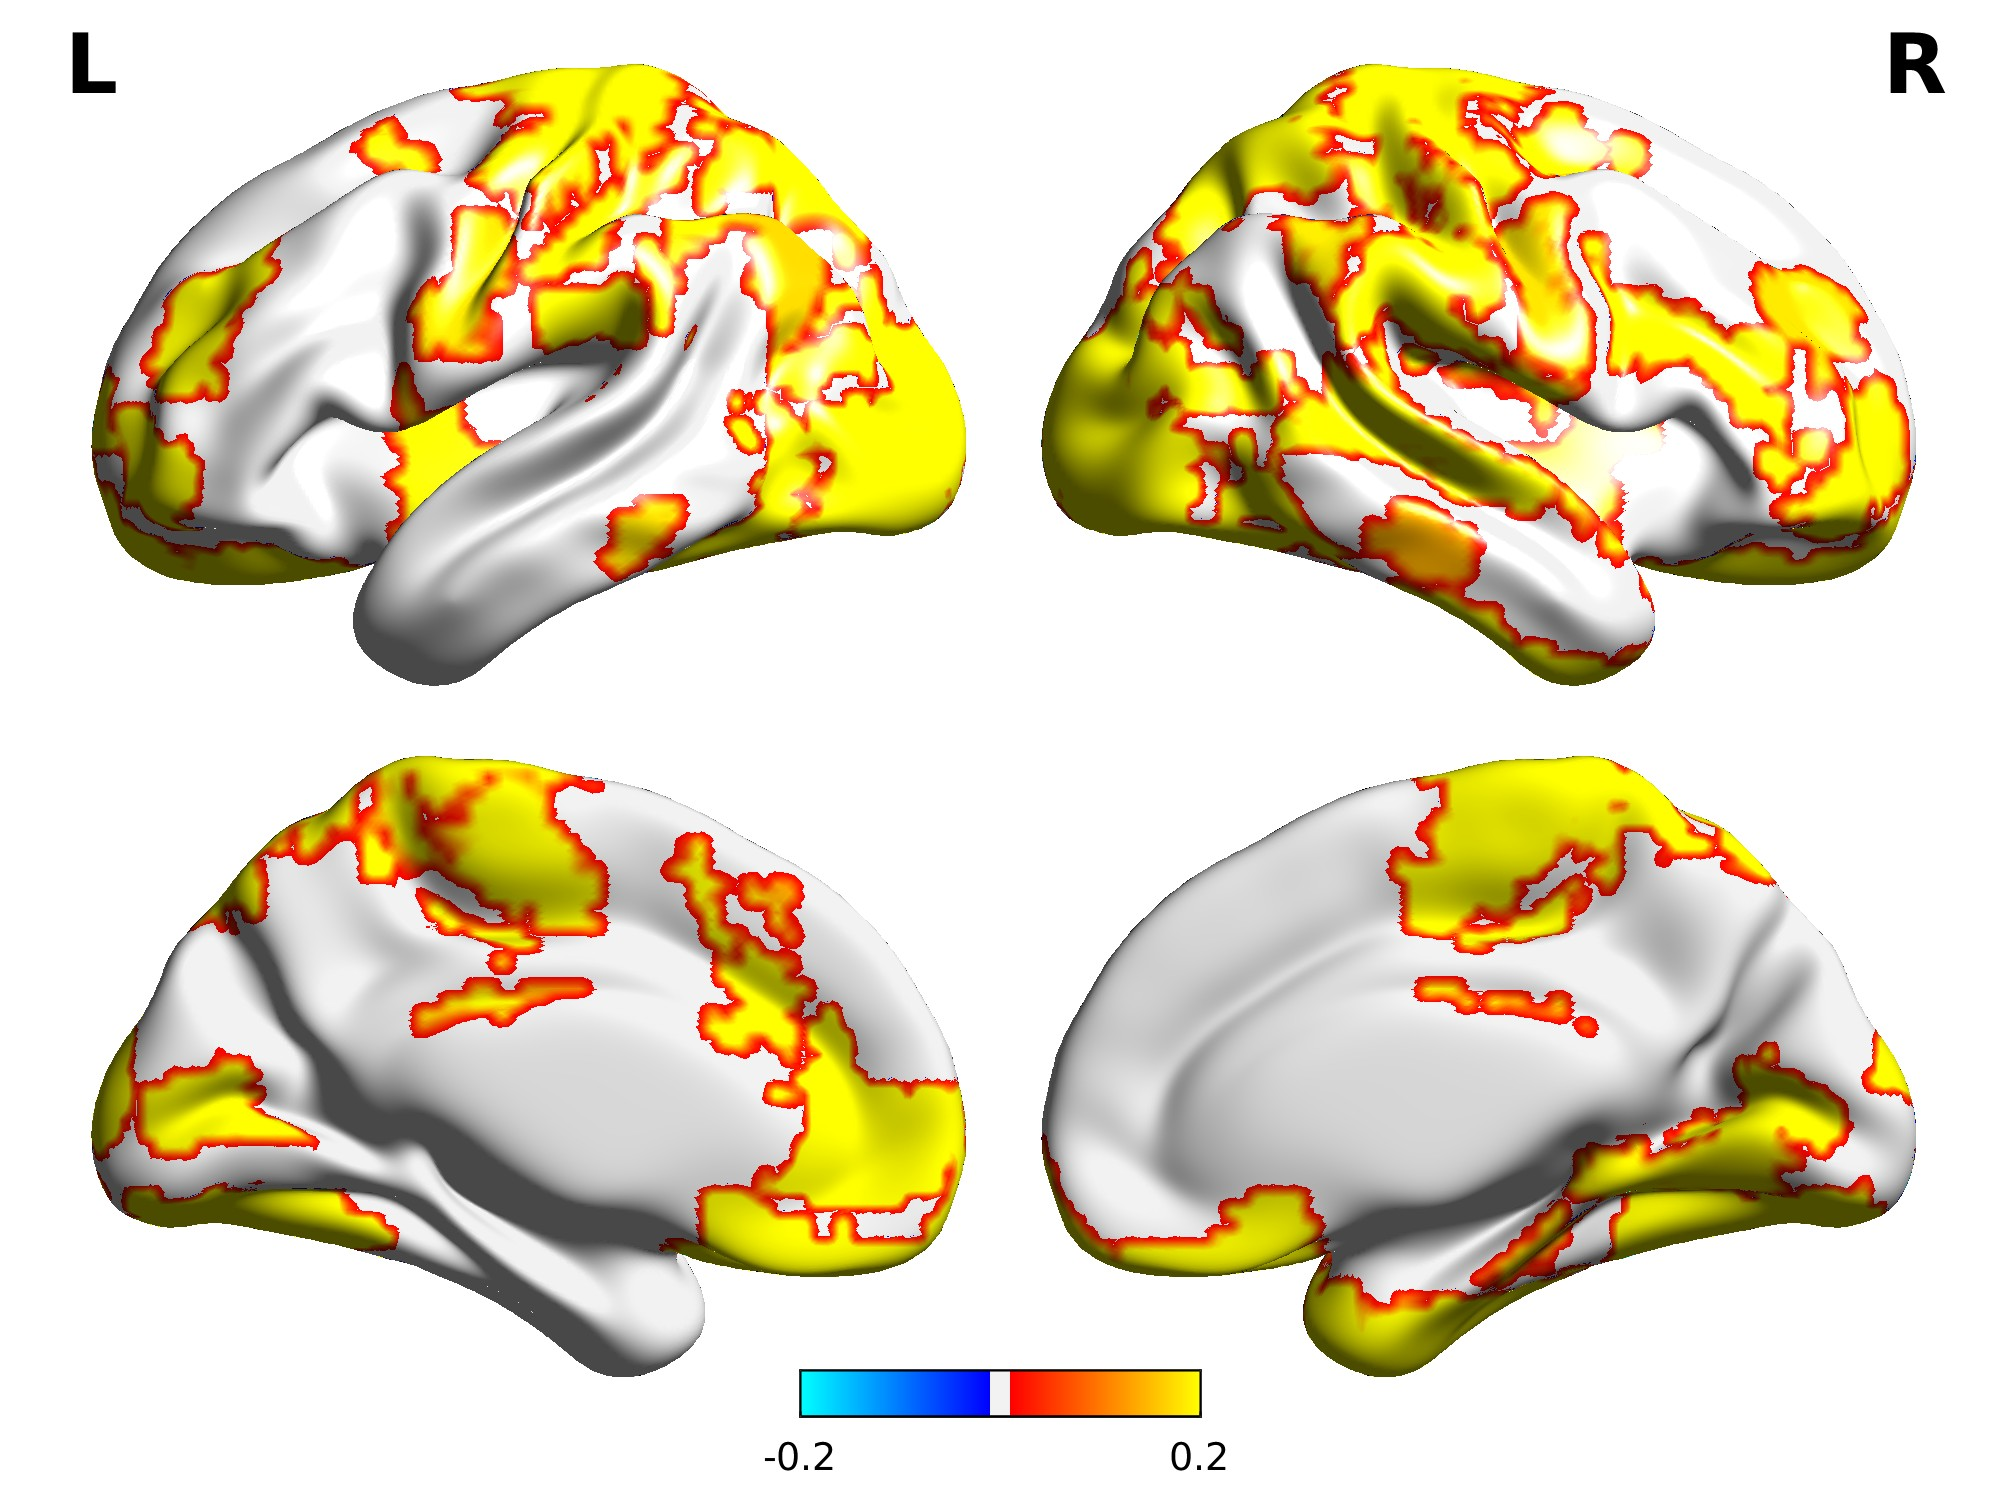
\includegraphics[width=0.85\textwidth]{figures/fig3a_grp_grp_r_pmasked.jpg}
    \caption{Brain surface map of aPCR prediction accuracy (group-level Pearson $r$, FDR-corrected significant ROIs highlighted). Brighter regions indicate ROIs where the model's predicted fMRI time series most closely tracks the observed fMRI. Of 122 ROIs, 56 are significantly predicted (FDR $q < 0.05$), with a median Pearson $r = 0.160$ across all ROIs.}
    \label{fig:brainmap}
\end{figure}

\subsubsection{Network-Level Breakdown}

Figure~\ref{fig:network} shows prediction accuracy broken down by functional network. The dorsal attention network (DAN) shows the strongest proportional performance: 11 of 14 ROIs are significantly predicted (79\%), the highest hit rate of any network. The ventral attention network (VAN) achieves 14 of 24 significant ROIs (58\%). The frontoparietal control network (CONT) reaches 12 of 26 (46\%), and the DMN reaches 6 of 26 (23\%). DAN's dominance is directly relevant to the individual differences hypothesis: DAN is the primary recruitment target of both n-back and CPT tasks \citep{owen2005}, and its strong performance in the training phase supports the expectation that the frozen model will capture task-evoked attention network dynamics.

The CONT performance is particularly encouraging given that this is a large, distributed network with 26 ROIs spread across medial and lateral surfaces, many of which are far from the fNIRS channels. That 12 ROIs survive FDR correction suggests the model is recovering network-level dynamics through temporal covariation rather than purely through direct cortical coverage. DMN performance (6/26) is lower than DAN and CONT, which may reflect reduced DMN engagement during movie-watching relative to resting state, or the fact that medial default-mode nodes are farther from the prefrontal-parietal fNIRS cap. Whether the DMN prediction holds up in task contexts, where DMN suppression is the theoretically predicted signal, is the central open question.

\begin{figure}[ht]
    \centering
    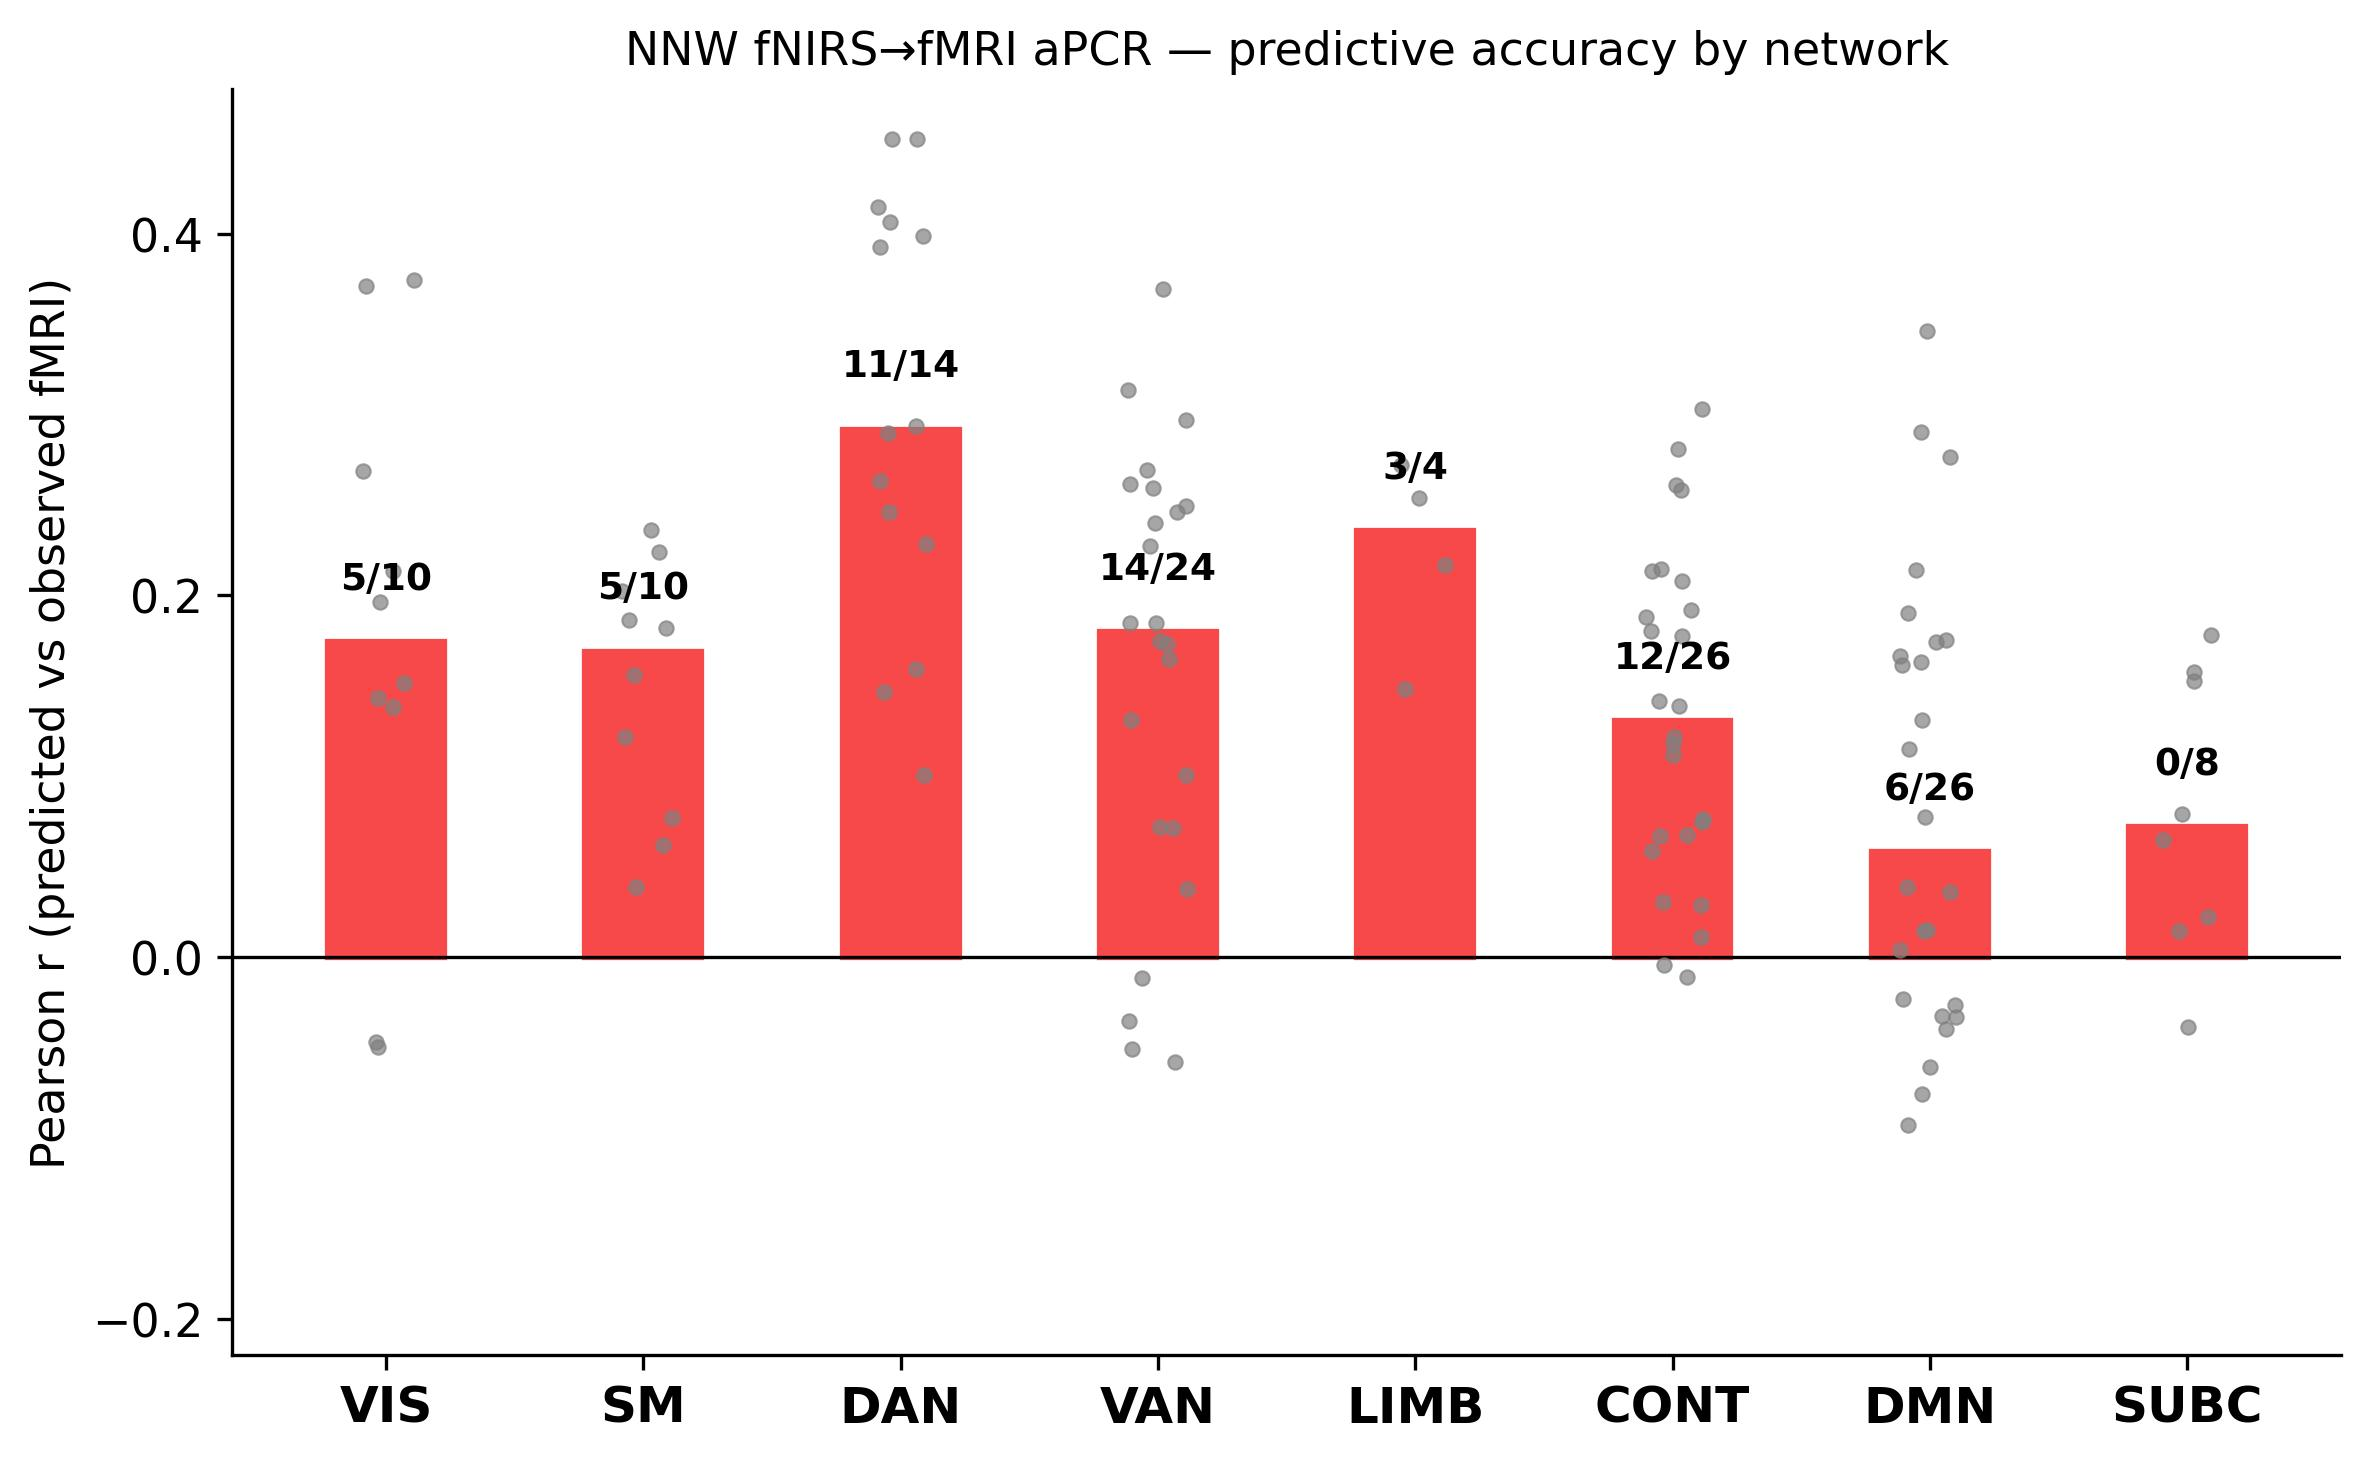
\includegraphics[width=0.85\textwidth]{figures/fig3b_network_barplot.jpg}
    \caption{aPCR prediction accuracy by functional network (Yeo 17-network + Brainnetome + subcortical atlas, collapsed to 8 systems). Bars show median Pearson $r$ across ROIs in each network; overlaid dots show individual ROI values. Fractions indicate the number of significantly predicted ROIs out of the total in each network (FDR $q < 0.05$): DAN 11/14, VAN 14/24, CONT 12/26, DMN 6/26, SM 5/10, VIS 5/10, LIMB 3/4, SUBC 0/8. Networks are ordered from posterior sensory to anterior/higher-order.}
    \label{fig:network}
\end{figure}

\subsubsection{Connectivity Structure Preservation}

The ISFC comparison addresses a question that per-ROI accuracy cannot: does the model preserve the large-scale organizational logic of the brain, not just isolated activation levels? Individual differences in attention are encoded in how networks communicate with one another, specifically in the dynamic balance between frontoparietal task-positive systems and the DMN \citep{cole2013, braun2015}. The Pearson correlation between the observed and predicted ISFC matrices (lower triangles) is $r = 0.617$ ($p = 0.001$, permutation test; Figure~\ref{fig:isfc}). The model is not just predicting individual regions; it is preserving the large-scale organization of how brain regions communicate during the movie. Both matrices show the expected anti-correlation between task-positive networks (DAN, VAN, CONT) and DMN, indicating the model captures the fundamental antagonistic relationship between these systems. This $r = 0.617$ value serves as the NNW benchmark against which cognitive task predictions will be compared.

\begin{figure}[ht]
    \centering
    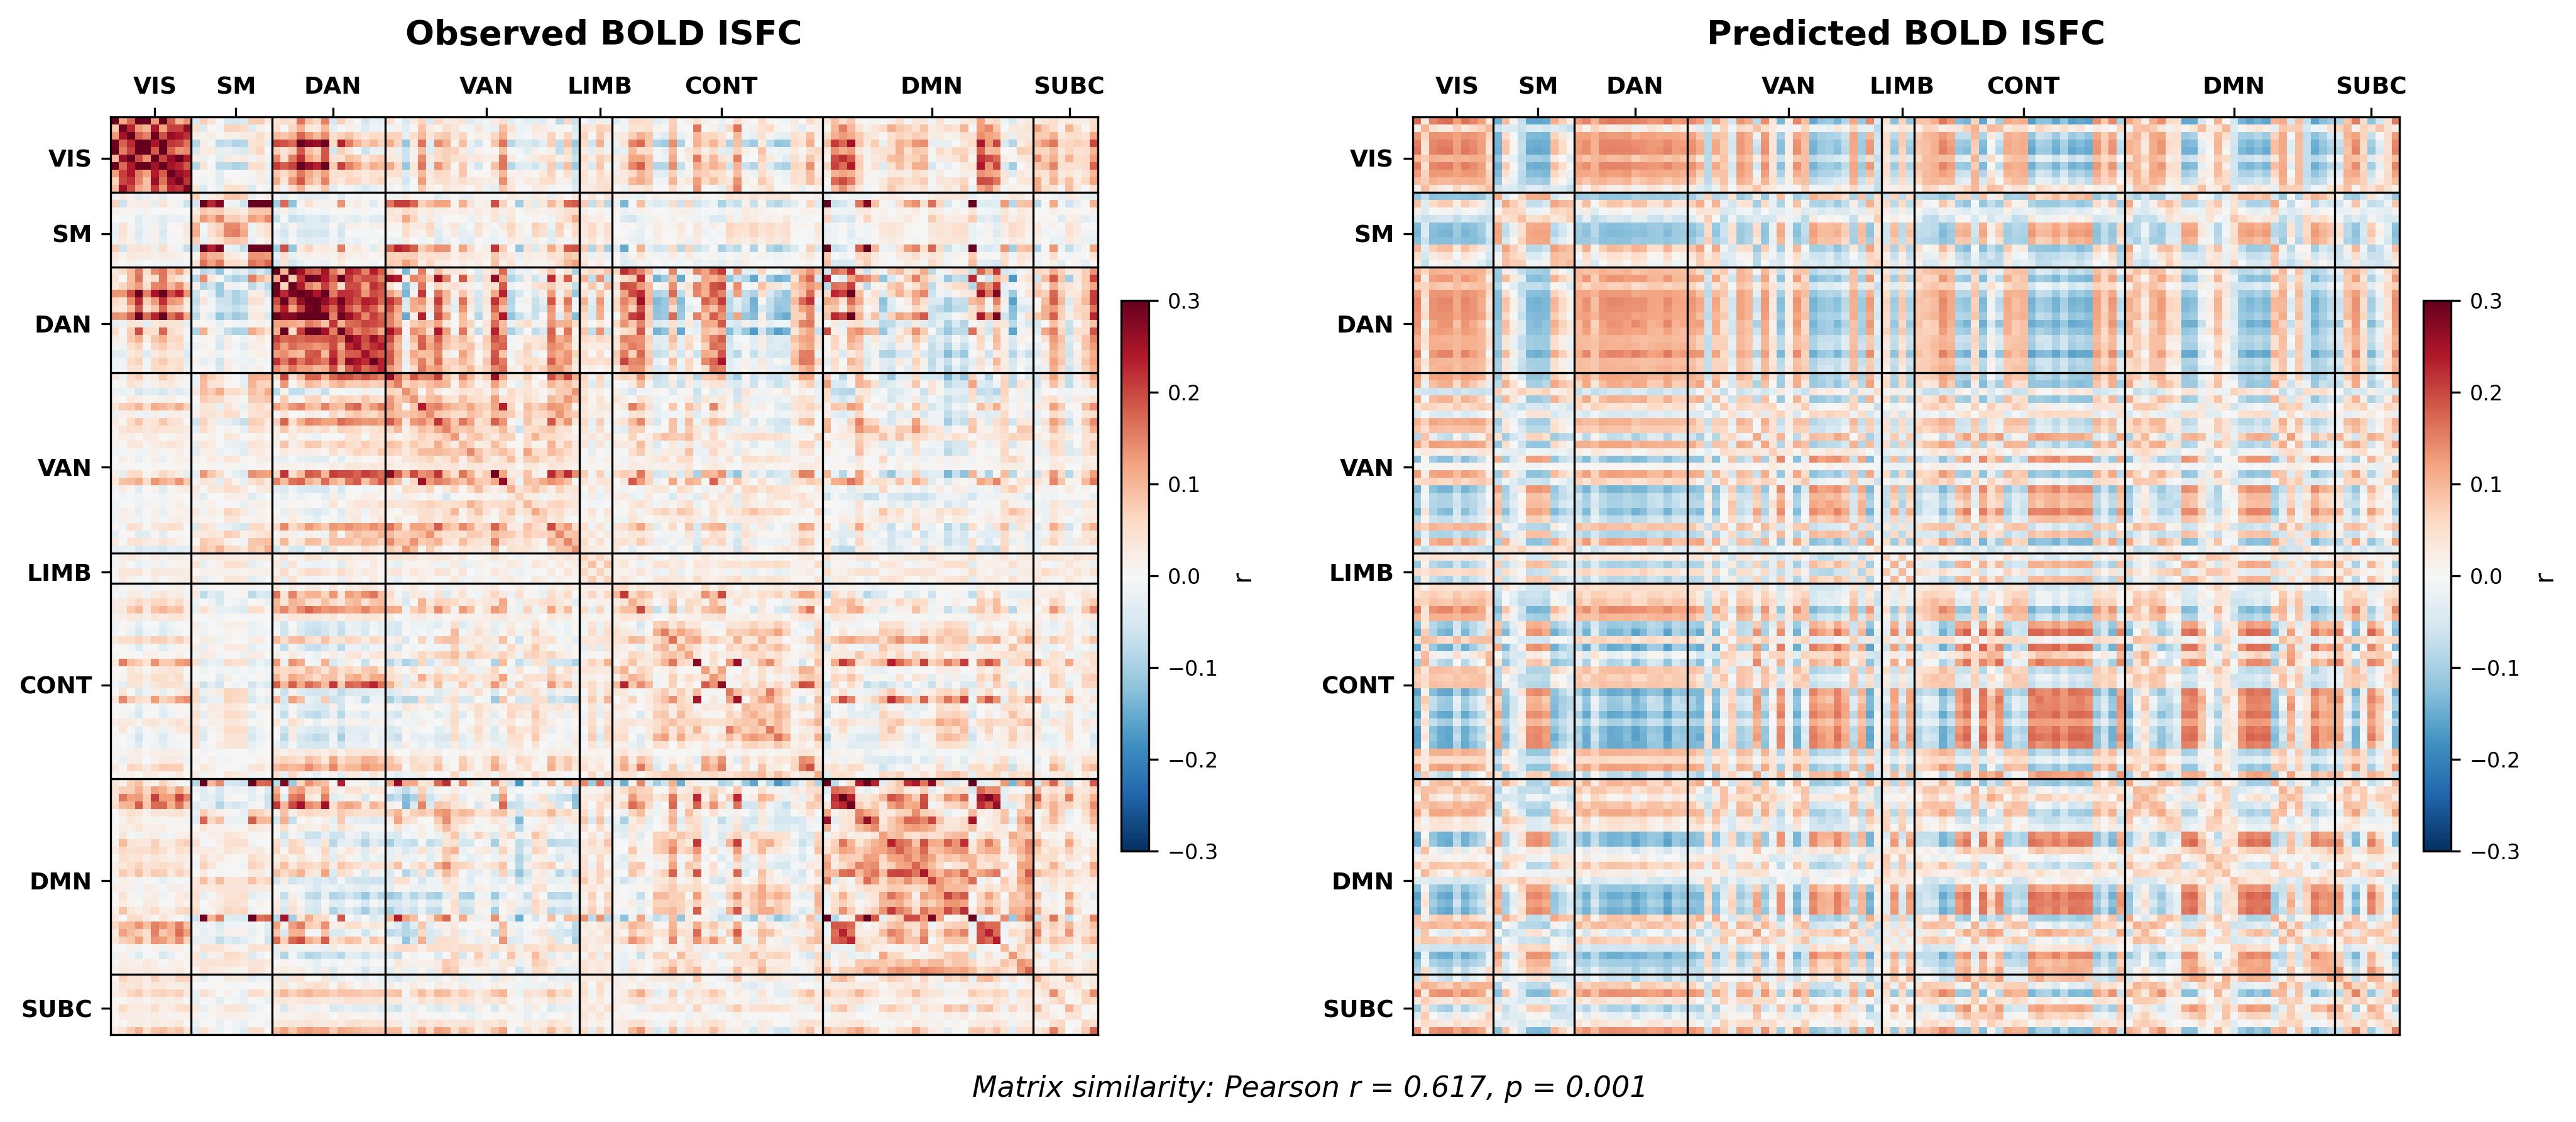
\includegraphics[width=\textwidth]{figures/fig4_isfc_heatmap.jpg}
    \caption{Observed versus predicted BOLD inter-subject functional connectivity (ISFC) matrices. Left: true fMRI ISFC. Right: ISFC reconstructed by the aPCR model from fNIRS signals alone. Each cell represents the average correlation between one ROI's time series and the leave-one-out group mean of another ROI, capturing how brain regions coordinate during the film. The Pearson correlation between the lower triangles of the two matrices is $r = 0.617$ ($p = 0.001$, permutation test).}
    \label{fig:isfc}
\end{figure}

\subsubsection{Independent Replication}

Applying the identical aPCR pipeline to a separate fNIRS dataset collected by a previous lab member (different participants, same NNW clip, same cognitive tasks) yielded 28 significantly predicted ROIs and an ISFC matrix similarity of $r = 0.297$ ($p = 0.001$). Both the number of significant ROIs and the ISFC similarity are lower than the primary dataset, likely reflecting differences in sample size and data quality. However, the result confirms the pipeline is not overfit to a single dataset.

An informative contrast emerges in the network-level pattern. In the replication dataset, the network ranking closely matches \citet{gao2025}: DMN and CONT lead in prediction accuracy. This differs from the primary dataset, where DAN dominates (11/14, 79\%) and CONT and DMN perform well but do not lead. One candidate explanation is task ordering: in the primary dataset, participants watched the movie at the end of a two-hour session after completing all cognitive tasks, whereas the replication dataset used a different session structure. If fatigue or reduced engagement selectively dampens narrative-driven DMN responses while leaving stimulus-driven visual responses intact, this could shift which networks the model predicts most accurately. Future data collection will place the movie-watching block first and include self-report measures of engagement and cap discomfort to test this possibility directly. Regardless of the mechanism, the fact that both datasets produce significant whole-brain predictions through different network emphases suggests the aPCR framework is robust, even if the specific network profile depends on recording conditions.


\subsection{Expected Results: Cross-Task Predictions and Individual Differences}

The preliminary results establish that the aPCR model captures real, network-level brain structure during movie-watching. The following analyses apply the frozen NNW model to cognitive task data and test whether the predictions carry behavioral meaning. These analyses are planned; the specific predictions below are grounded in the existing literature and in the pattern of results from the training phase.

\subsubsection{Expected Result 1: Cross-Task Neural Plausibility}

When the frozen NNW model is applied to n-back fNIRS data, the predicted fMRI time series should show task-appropriate activation patterns even though the model has never encountered structured cognitive tasks. Three specific predictions follow from the fMRI literature on working memory:

First, predicted activation in DAN and CONT ROIs should be higher during 2-back blocks than during 1-back blocks. The n-back task is the most extensively studied working memory paradigm in fMRI, and the meta-analysis by \citet{owen2005} identifies bilateral dorsolateral prefrontal cortex, premotor cortex, and posterior parietal cortex (all within DAN and CONT) as the regions most consistently recruited by increasing working memory load. If the frozen model captures generalizable cortical-subcortical relationships, the predicted activation in these regions should track load even without any task-specific training.

Second, predicted DMN activation should show the inverse pattern: lower activation during 2-back than during 1-back. DMN suppression during cognitively demanding tasks is one of the most replicated findings in the fMRI literature \citep{sonugabarke2007}, and the degree of suppression scales with task difficulty. The model's ability to predict this pattern from surface fNIRS signals would provide strong evidence that the learned mapping captures the antagonistic relationship between task-positive and task-negative systems.

Third, ISFC computed on the predicted cognitive-task fMRI should be lower than the NNW benchmark ($r = 0.617$) but significantly above chance. ISC values near zero are expected for trial-based, non-naturalistic paradigms because individual differences in strategy, arousal, and performance make neural responses less consistent across participants \citep{nastase2019}. A meaningful but attenuated ISFC would indicate that the model is capturing whatever shared structure exists in the task data rather than producing noise.

I will quantify these patterns using paired $t$-tests comparing predicted ROI activation between 1-back and 2-back blocks, computed separately for each functional network. Effect sizes (Cohen's $d$) will be reported alongside significance to characterize the magnitude of any load-dependent differences the model detects.

\subsubsection{Expected Result 2: Behavioral Correlates of Predicted Neural Patterns}

The central individual-differences hypothesis is that predicted brain patterns should correlate with how well participants actually perform the cognitive tasks. The analyses are organized around three behavioral measures: reaction time variability, task accuracy, and signal detection sensitivity.

\paragraph{Reaction time variability and DMN dynamics.} The most theoretically grounded prediction concerns the relationship between predicted DMN activation and reaction time variability (RTV). RTV is computed as the intraindividual standard deviation of correct-trial reaction times (iSD-RT) within each participant for each task and load condition. During goal-directed tasks, the DMN is normally suppressed; when suppression fails periodically, the DMN reactivates and disrupts processing, producing attentional lapses that manifest as unusually slow, variable responses \citep{sonugabarke2007, kofler2013}. The prediction is directional: participants with higher predicted DMN mean activation during the n-back should show higher RTV (Figure~\ref{fig:dmn_rtv}).

I will test this with Pearson correlations between per-subject predicted DMN mean activation (averaged across the 26 DMN ROIs and across task blocks) and per-subject iSD-RT, computed separately for 1-back and 2-back conditions. The expected effect size is $r \approx 0.35$ to $0.45$, attenuated from published fMRI-behavior correlations ($r \approx 0.50$ to $0.60$; \citealp{braun2015, finn2021}) to account for the information loss inherent in model-predicted rather than directly measured fMRI. At the current sample size (N\,=\,28), effects in the $r \approx 0.40$ range are detectable but underpowered for stringent correction. The project targets N\,=\,40, at which effects of this magnitude achieve approximately 80\% power.

The same analysis will be run using the coefficient of variation of RT (CV-RT\,=\,SD/Mean) as an alternative operationalization of RTV. CV-RT controls for differences in mean RT across participants, which matters if some participants adopt a generally slower response strategy rather than experiencing genuine attentional lapses. If both iSD-RT and CV-RT correlate with predicted DMN activation in the same direction, this strengthens the interpretation that the model is capturing DMN-mediated attentional instability rather than overall response speed.

\begin{figure}[ht]
    \centering
    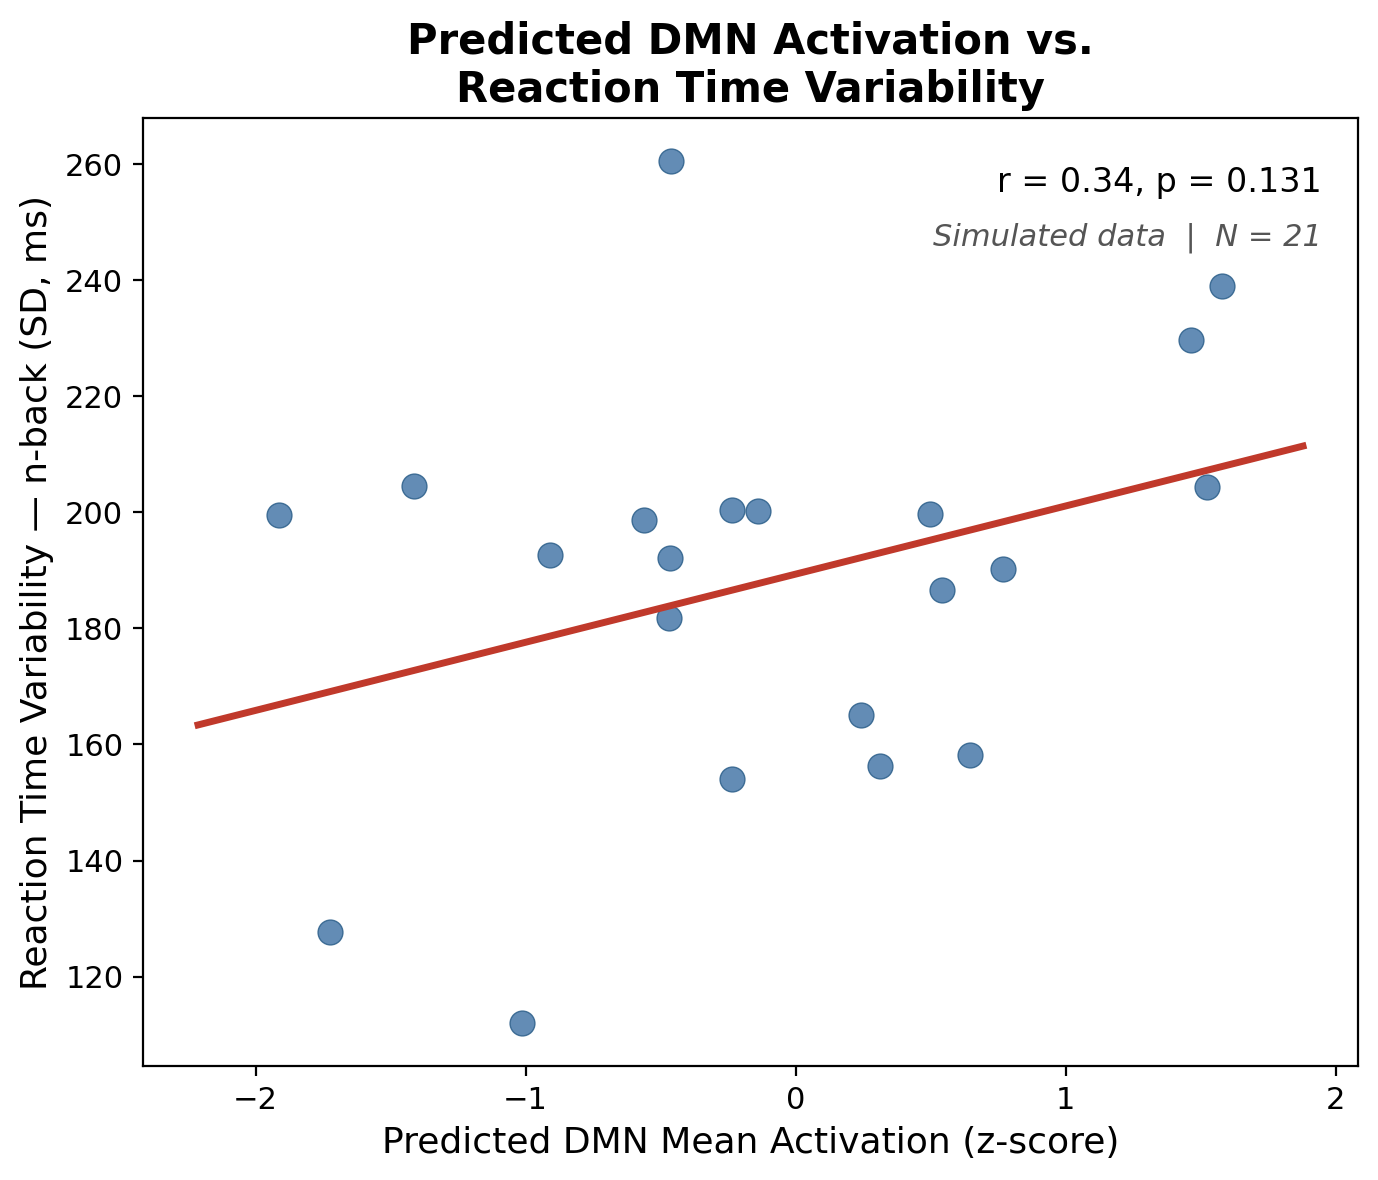
\includegraphics[width=0.65\textwidth]{figures/fig_mockup_dmn_rtv.png}
    \caption{Simulated data. Expected relationship between predicted DMN mean activation during the n-back task and reaction time variability (SD of response times across trials). Data were simulated for N\,=\,28 participants using a target correlation of $r = 0.40$, consistent with the hypothesis that greater DMN intrusion during task performance is associated with more variable response times. Predicted DMN activation was drawn from a standard normal distribution; RTV was generated as a linear combination of DMN activation and independent noise, scaled to realistic n-back RT distributions (mean SD $\approx$ 200\,ms, range $\approx$ 120--280\,ms). This figure illustrates the expected direction and approximate magnitude of the effect; actual values will depend on cognitive task preprocessing results.}
    \label{fig:dmn_rtv}
\end{figure}

\paragraph{Task accuracy and frontoparietal engagement.} Beyond RTV, I will test whether predicted DAN and CONT mean activation during n-back blocks correlates with n-back accuracy (proportion correct, computed separately for 1-back and 2-back). The literature predicts positive correlations: participants whose frontoparietal networks show greater task-evoked reconfiguration tend to perform better on working memory tasks \citep{braun2015, cole2013}. The expected effect size is smaller than the DMN-RTV relationship ($r \approx 0.25$ to $0.35$), and ceiling effects in 1-back accuracy (where most healthy young adults score near-perfect) may limit the sensitivity of this analysis in the 1-back condition. The 2-back condition, which produces more variance in accuracy, is the stronger test.

\paragraph{CPT signal detection and sustained attention.} For the CPT, I will compute d-prime and criterion from hit and false alarm rates (with a 0.5-trial correction for boundary cases) and correlate these with predicted mean activation in DAN and CONT. RTV from the CPT will also be computed and correlated with predicted DMN activation, replicating the n-back analysis in a sustained attention context. Consistent DMN-RTV correlations across both n-back and CPT would strengthen the case that the model captures a domain-general attentional stability mechanism rather than task-specific variance.

\subsubsection{Expected Result 3: Load-Dependent Prediction Quality}

Comparing prediction quality across conditions that differ in cognitive load will reveal whether the naturalistic mapping captures dynamics that scale with task demands. Specifically, I will compute per-ROI prediction variance explained ($R^2$) separately for 1-back and 2-back blocks and compare them using paired $t$-tests across the 56 significant NNW ROIs. Two outcomes are possible, and each is informative:

If prediction quality is comparable across load levels, this suggests the NNW-trained mapping captures a stable cortical-subcortical relationship that persists regardless of cognitive demand, supporting the case for naturalistic calibration as a universal tool. If prediction quality degrades with increasing load, this would indicate that the mapping captures baseline and low-demand dynamics better than executive-control dynamics, establishing a meaningful boundary condition on the approach. Either result advances the field's understanding of when and where naturalistic calibration works.

\subsubsection{Summary of Planned Statistical Tests}

Table~\ref{tab:tests} summarizes the planned analyses, specifying the predictor, outcome, and expected direction for each test.

\begin{table}[ht]
\centering
\small
\caption{Planned individual-differences analyses. All correlations are Pearson $r$, computed across subjects separately for each task and condition. FDR correction is applied across tests within each family.}
\label{tab:tests}
\begin{tabular}{p{3.5cm} p{3.5cm} p{2.5cm} p{2.5cm}}
\hline
\textbf{Neural predictor} & \textbf{Behavioral outcome} & \textbf{Expected direction} & \textbf{Task/condition} \\
\hline
Predicted DMN mean activation & iSD-RT (RTV) & Positive ($r \approx 0.40$) & n-back 1B, 2B \\
Predicted DMN mean activation & CV-RT & Positive & n-back 1B, 2B \\
Predicted DAN mean activation & Accuracy (\% correct) & Positive ($r \approx 0.30$) & n-back 2B \\
Predicted CONT mean activation & Accuracy (\% correct) & Positive & n-back 2B \\
Predicted DAN mean activation & d-prime & Positive & CPT \\
Predicted DMN mean activation & iSD-RT (RTV) & Positive & CPT \\
2B--1B predicted DAN contrast & 2B--1B accuracy change & Positive & n-back \\
\hline
\end{tabular}
\end{table}

 
% --- Discussion ---
% discussion.tex — Full proposal draft, Week 8
% Synthesized from Week 4 evaluation and Week 7 limitations, with new framing.

\section{Discussion}

\subsection{What the Preliminary Results Establish}

The NNW training phase establishes three things that are necessary before the cross-task analyses can proceed. First, the aPCR model significantly predicts 56 of 122 brain regions during naturalistic movie-watching, demonstrating that whole-brain fMRI dynamics can be recovered from surface fNIRS signals in a dataset where fNIRS and fMRI were recorded from entirely different people. Second, the predicted connectivity structure closely matches the observed connectivity structure ($r = 0.617$), which means the model is not just predicting isolated regions but preserving the large-scale organizational logic of the brain, including the antagonistic relationship between task-positive and default-mode networks. Third, the networks most relevant to the individual-differences hypothesis (DAN, CONT, DMN) are among the best-predicted, with 29 of 56 significant ROIs falling in these three systems. This pattern is consistent with the fact that these networks are the most consistently engaged by the narrative structure of a film \citep{hasson2010} and are therefore the networks where the cross-participant, cross-modality alignment is strongest.

\subsection{Interpreting the Network Ranking Discrepancy}

One finding that requires careful interpretation is that the network-level prediction profile in the primary dataset differs from both the \citet{gao2025} framework and an independent replication dataset collected in the same lab. In the replication dataset, DMN and CONT lead in prediction accuracy, consistent with Gao et al.'s results using BBC \textit{Sherlock}. In the primary dataset, VIS and DAN lead, with DMN and CONT performing well but not dominating. Both datasets produce significant whole-brain predictions with meaningful ISFC, but they emphasize different networks.

A plausible explanation involves session ordering and time-on-task effects. In the primary dataset, participants watched NNW at the end of a two-hour session after completing all cognitive tasks. A well-established literature on time-on-task effects shows that prolonged cognitive effort alters the dynamic balance between task-positive and default-mode networks: sustained attention depletes executive resources and reduces the efficiency of DMN suppression and reactivation \citep{sonugabarke2007}. If fatigue selectively dampens narrative-driven DMN engagement with the film (because tired participants track the story less deeply) while leaving stimulus-driven visual and attentional responses relatively intact (because bottom-up processing of visual action sequences requires less effortful engagement), this would shift the network profile toward VIS and DAN without degrading overall prediction accuracy. The replication dataset, which used a different session structure, would not show this shift, explaining why it reproduces the Gao et al.\ pattern.

This interpretation has a testable implication. Future data collection will place the movie-watching block first in the session, before any cognitive tasks, and will include self-report measures of engagement and cap discomfort. If the movie-first ordering restores the DMN/CONT-dominant pattern, that would confirm that session ordering modulates which networks the model predicts best. This also has practical consequences for the individual differences analyses in Phase 5: the DMN-RTV hypothesis depends on the model's ability to predict DMN dynamics during cognitive tasks. If DMN prediction is attenuated in the primary dataset due to training-phase fatigue effects, the DMN-RTV correlation may be weaker than expected, making the movie-first design change important for maximizing the sensitivity of the individual differences test.

\subsection{Why the Cross-Task Test Is Meaningful}

The most principled aspect of this design is using movie-watching as the training stimulus rather than a structured task. The whole analysis depends on having temporally consistent brain responses across both fNIRS and fMRI participants, and naturalistic stimuli are what produce that consistency \citep{hasson2010, nastase2019}. Structured cognitive tasks could not serve this role because individual differences in performance, strategy, and arousal make brain responses too person-specific to train a cross-dataset model. So the design is not using movie-watching out of convenience; it is using it because it is the paradigm that best supports cross-person, cross-modality model training. The whole logic of the project is to calibrate on shared signal, then test on individual variation.

The frozen-model design also directly addresses what would otherwise be an insurmountable practical constraint: there is no cognitive-task fMRI dataset from the same people who did the fNIRS cognitive tasks. Rather than treating this as a problem, the design frames it as the test itself: does a model calibrated on passive movie-watching transfer to structured cognitive tasks? The NNW results show the model produces coherent predictions in the training domain, which justifies testing cross-task transfer.

\subsection{Limitations}

Several limitations should be noted.

The main limitation is spatial coverage. The fNIRS cap covers prefrontal and lateral parietal cortex but has no channels over medial prefrontal cortex, primary visual cortex, or subcortical areas. The model's ability to predict those regions during cognitive tasks rests entirely on statistical covariation patterns learned from the movie. The NNW results show this can work (VIS and SM are significantly predicted despite no direct coverage), but the mechanism is likely shared temporal dynamics during the movie, not true spatial fidelity. This is an important caveat for any ROI-level interpretation of cognitive task predictions.

Sample size is a concern. N\,=\,28 for the NNW model is enough to test the pipeline, but the individual differences regression in Phase 5 will struggle to detect effects smaller than $r \approx 0.40$ at this sample size. The plan is to keep recruiting toward N\,=\,40, and to report effect sizes and confidence intervals rather than relying solely on significance, so the results are interpretable regardless of where the final sample lands.

There is no cognitive-task fMRI ground truth to directly validate the predictions against. The validation strategy, checking ISFC, comparing against the n-back literature, and correlating with behavior, is indirect but informative. Each of these provides a different kind of evidence that the predictions are meaningful, and together they make a reasonable case even without matched fMRI data. External validation against large public fMRI datasets (HCP n-back, N\,=\,1,200; DMCC AX-CPT, N\,=\,55) remains an option if the within-sample correlations are too underpowered.

Finally, the behavioral data quality issues described in the Methods (duplicate files, accuracy coding verification, CPT metric recomputation) must be resolved before the individual differences analyses can be run. These are bookkeeping problems, not conceptual ones, but they need to be completed before Phase 5 proceeds.

\subsection{Why This Is the Right Approach}

The obvious alternative would be to collect fMRI and fNIRS simultaneously during cognitive tasks from the same participants and train the model directly on that data. This would solve the spatial validation problem and eliminate the frozen-model assumption. But it also requires every participant to go in the scanner, which is the exact problem the project is trying to solve. If scanner access is required, there is no scalable, equitable version of this tool.

The naturalistic training design trades direct validation for accessibility, and that tradeoff is the whole point of the project. The NNW results show the model is not noise; it captures real structure during the training condition. The cognitive task analyses will tell us how much of that structure persists when the context changes. Whatever the answer is, it moves the field forward on a question that matters both scientifically and practically.

Even a null result has scientific value. If the frozen model fails to predict cognitive-task brain patterns or fails to correlate with attention performance, that is a meaningful boundary condition on the approach, not just a failed experiment. It would tell us something specific about when naturalistic calibration does and does not generalize, which is useful for the broader goal of portable neurocognitive assessment \citep{farah2006, noble2015}.

\subsection{Broader Implications}

If the cross-task predictions succeed, the practical implications extend well beyond this study. A portable fNIRS session lasting under 15 minutes (the NNW clip), requiring no scanner, no special infrastructure, and no trained MRI technician, would be sufficient to calibrate a model that then provides whole-brain-equivalent neural measures during any subsequent cognitive assessment. This opens the possibility of neurocognitive research in schools, community clinics, field settings, and populations that have been structurally excluded from scanner-based science. The equity argument runs through every design choice in this project, from the use of a shared movie stimulus that requires no literacy or cultural familiarity, to the focus on individual differences in attention that track socioeconomic and clinical disparities, to the explicit goal of building a tool that works without the infrastructure that currently gatekeeps access to brain science \citep{burns2019, farah2006}.

 
% --- Conclusion ---
% conclusion.tex — Full proposal draft, Week 8

\section{Conclusion}

This project tests whether a brief, portable brain recording session, calibrated on naturalistic movie-watching, can serve as a window into whole-brain neural dynamics during structured cognitive tasks and into individual differences in attentional control. The preliminary results from the movie-watching training phase show that the aPCR model recovers large-scale brain organization from fNIRS surface signals alone, with significant prediction in 56 of 122 brain regions and strong preservation of inter-network connectivity structure ($r = 0.617$). The dorsal attention network (DAN) shows the strongest proportional performance (11 of 14 ROIs, 79\%), with the frontoparietal control network and default mode network also significantly predicted, providing a foundation for the cross-task individual differences analyses. If those analyses show that predicted brain patterns correlate with reaction time variability and task performance, the result would be a candidate method for conducting whole-brain-equivalent neurocognitive assessment without a scanner, with direct implications for making attention research accessible to the populations and settings where it is needed most.

 
% --- Data Availability ---
% data_availability.tex — Full proposal draft, Week 8

\section{Data Availability and Reproducibility}

All analysis code for this project is publicly available at \url{https://github.com/judycchen/30200_proposal}. The repository is organized as a numbered pipeline: fMRI ROI extraction (step a), fNIRS preprocessing and exclusion (steps b1--b2), fNIRS-fMRI spatial correlation and control analyses (steps c--c3), MNI brain visualization (step d), aPCR model training and prediction (step e), permutation-based significance testing (step f), ISFC analysis (step g), and ROI and network visualization (steps h--i). Each step has a matching Slurm batch submission file for execution on the University of Chicago Research Computing Center's Midway3 cluster. Python dependencies include NumPy, scikit-learn, nibabel, nilearn, and BrainIAK; MATLAB scripts use the NIRS Brain AnalyzIR Toolbox \citep{santosa2018}.

The fNIRS data were collected under an approved IRB protocol at the University of Chicago and will be made available upon reasonable request following study completion, in accordance with institutional data sharing policies. The fMRI dataset (N\,=\,59, NNW movie-watching) was obtained from a collaborating lab and is available through the original data sharing agreement. Preprocessed behavioral data (trial-level reaction times and accuracy) will be shared alongside the analysis code upon publication. Preprocessed fNIRS data are excluded from the repository due to file size and are stored on the Midway3 cluster.


 
% --- References ---
\printbibliography
 
\end{document}